\documentclass[12pt]{article}
\usepackage{amsfonts, epsfig}
\usepackage[authoryear]{natbib}
\usepackage{graphicx}
\usepackage{fancyhdr}
\pagestyle{fancy}
\lfoot{\texttt{comsm0021.github.io}}
\lhead{Neural Information Processing - 8\_forward\_models - Conor}
\rhead{\thepage}
\cfoot{}
\begin{document}

\section*{A forward model for the perception of movement}

In neuroscience, and in control theory, a \textsl{forward model} is an
internal model responsible for what performing calculations analagous
to the dead reckoning discussed in the context of Kalman filters.

A well-known discussion of forward models in given in
\cite{WolpertEtAl1995}. In this paper they give some, albeit quite
circumstantial, evidence that the brain has a forward model for
movement. In their experiment subjects are sat in the dark with one
hand on a manipulandum, that is, a device you push around with one
hand which can record your hand, restrict it to specific paths and
excert a force against or with the movement of your hand. A
manipulandum is shown in Fig.~\ref{fig_manipulandum}.

In this experiment the manipulandum is restricted to horizonal
motion. At the start of each trial the subjects hand is illuminated so
that the subject knows where their hand is. The subject is then asked
to move their hand; there may be a force assisting or resisting this
movement, in any case at the end a restiance force is used to force
the subject to stop moving there hand at a point uniformly chosen
between zero and 30 cm.  The subject is then asked to use their other
hand to indicate, using a mouse which moves a marker along the
horizonal track, where they believe where their hand is. It turns our
people consistiently over-estimate how far their hand has
travelled.\footnote{This raises a plethora of questions; like if they
  then get visual feedback does the estimate improve? Is the
  overestimate the result of not modelling the braking force? This
  isn't dealt with in the paper and may work against its conclusions!}
In fact this overestimate has a distinctive timecourse shown in
Fig.~\ref{fig_overestimate}: the overestimate increases rapidly for
movements that take a second or less and then descreases slowly for
longer movements.


\begin{figure}{htb}
\begin{center}
  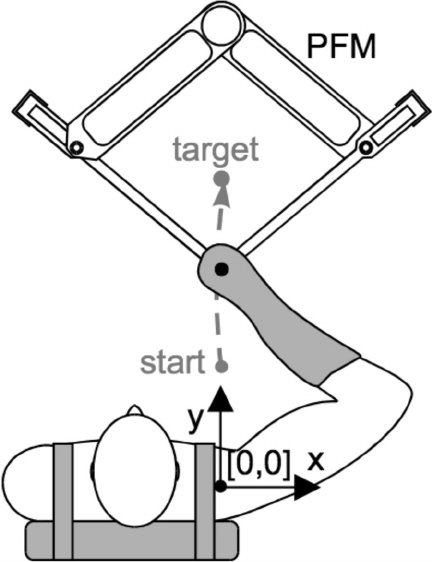
\includegraphics[width=6cm]{manipulandum.jpg}
\end{center}
\caption{A manipulandum allows hand movements to be recorded and to be manipulated by applying a force. [Image from \cite{MistryEt2013}, the start and target labels don't apply to the experiment being discussed here].\label{fig_manipulandum}}
\end{figure}


\begin{figure}{htb}
\begin{center}
  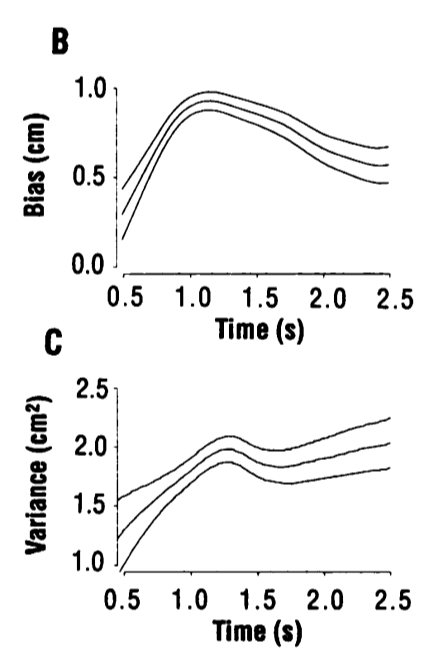
\includegraphics[width=5cm]{fig_overestimate.png}
\end{center}
\caption{The bias in estimates of hand position; \textbf{B} shows the
  mean bias and \textbf{C} the mean variance. The middle line shows
  the mean and the two outer lines are standard errors indicating the
  variability of the measurement. The participants never stop moving their hands in less than 0.5 seconds so the graphs start there; after 2.5 second the bias stops changing; 1 second corresponds to 0.9 cm and 2.5 seconds to 2 cm. [Image from
    \cite{WolpertEtAl1995}].\label{fig_manipulandum}}
\end{figure}

It is proposed in \cite{WolpertEtAl1995} that this is evidence for a
forward model. In there description the sense of hand position in the
absence of visual feedback has two components, a dead reckoning
component supplied by the forward model and a proprioceptive component
coming from mechano-receptors in the arm itself.


\bibliographystyle{apa} \bibliography{../../source/bibliography}{}



\end{document}

